%%%%%%%%%%%%%%%%%%%%%%%%%%%%%%%%%%%%%%%%%%%%%%%%%%%%%%%%%%%%%%%%%%%%%%%%%%%%%%%%%%%%%
\section{Introduction} \label{sec:gd_intro}
%%%%%%%%%%%%%%%%%%%%%%%%%%%%%%%%%%%%%%%%%%%%%%%%%%%%%%%%%%%%%%%%%%%%%%%%%%%%%%%%%%%%%

The field of astrophysics now has several instruments and observatories sensitive to high energy gamma-rays.
The energy sensitivity for the modern gamma-ray program spans many orders of magnitude.
\Cref{fig:gd_motivation} demonstrates these similar sensitivities across energies for the five experiments: Fermi-LAT, HAWC, HESS, MAGIC, and VERITAS.

\begin{figure}[t]
    \centering{
        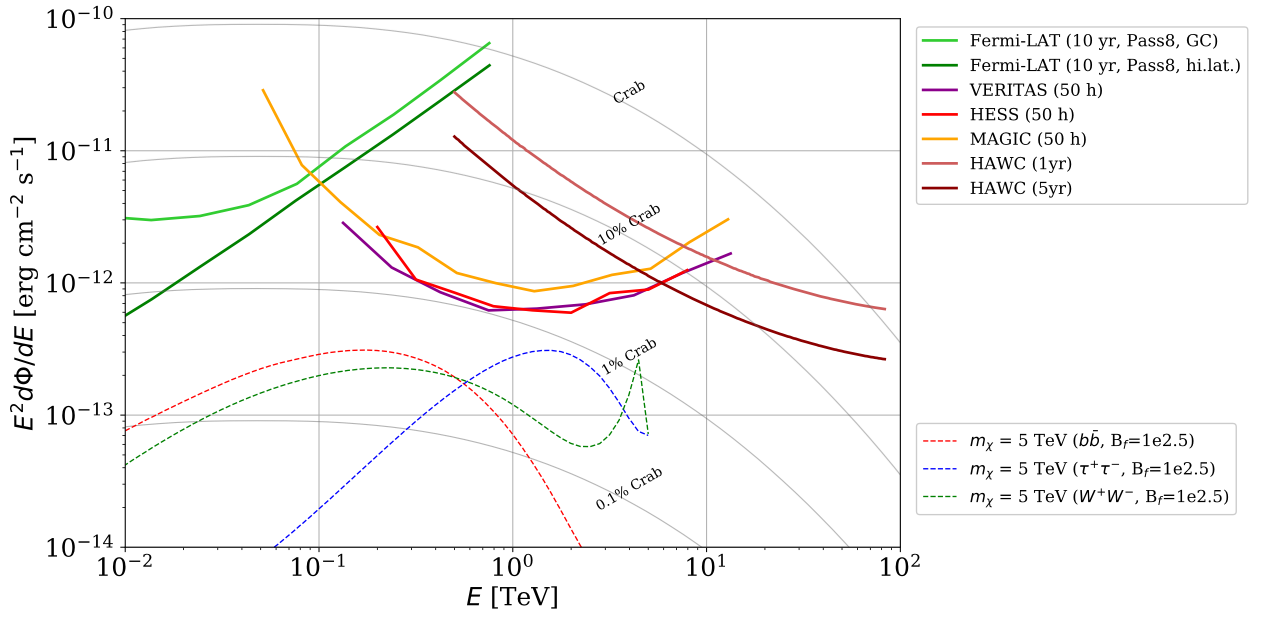
\includegraphics[scale=0.35]{figures/glory_duck/gd_motivation.png}
    }
    \caption{Sensitivities of five gamma-ray experiments compared to percentages of the Crab nebula's emission and dark matter annihilation. Solid lines present estimated sensitivities to power law spectra \fu for each experiment. Green lines are Fermi-LAT sensitivities where lighter green is the sensitivity to the galactic center and dark green is its sensitivity to higher declinations. Orange, red, and purple solid lines represent the MAGIC, HESS, and VERITAS 50 hour sensitivities respectively. The maroon and brown lines are the HAWC 1 year and 5 year sensitivities. Across four decades of gamma-ray energy, these experiments have similar sensitivities on the order $10^{-12}$ erg cm$^{-2}$s$^{-1}$. The dotted lines are estimated dark matter fluxes assuming $m_{\chi} = 5$~TeV DM annihilating to bottom quarks (red), tau leptons (blue), and W bosons (green). Faded gray lines outline percentage flux of the Crab nebula. Figure is an augmented version of \cite{2020Galax...8...25R}}
    \label{fig:gd_motivation}
\end{figure}

Each of the five experiments featured in \Cref{fig:gd_motivation} have independently searched for DM annihilation from dwarf spheroidal galaxies (dSph) and set limits.
Intriguingly, there are regions of substantial overlap in their energy sensitivities.
This clearly motivates an analysis that combines data from these five.
Each experiment has unique gamma-ray detection methods and their weaknesses and strengths can be leveraged with each other.
The HAWC gamma-ray observatory is extensively introduced in \Cref{sec:hawc}, so it is not introduced here.
A brief description of the remaining experiments are in the following paragraphs.

The Large Area Telescope (LAT) is a pair conversion telescope mounted on the NASA Fermi satellite in orbit $\sim$550 km above the Earth \cite{FermiLAT}.
LAT's field of view covers about 20\% of the whole sky, and it sweeps the whole sky approximately every 3 hours.
LAT's gamma-ray energy sensitivity ranges from 20 MeV up to 1 TeV.
Previous DM searches towards dSphs using Fermi-LAT are published in \cite{FermiLAT:dm1} and \cite{FermiLAT:dm2}

\sloppy The High Energy Spectroscopic System (HESS), Major Atmospheric Gamma Imaging
Cherenkov (MAGIC), and Very Energetic Radiation Imaging Telescope Array System (VERITAS) are arrays of Imaging Atmospheric Cherenkov Telescopes (IACT).
These telescopes observe the Cherenkov light emitted from gamma-ray showers in the Earth's atmosphere.
The field of view for these telescopes is no larger than $5\degree$ with energy sensitivities ranging from ~ 30 GeV up to 100 TeV \cite{HESS,MAGIC,VERITAS}.
IACTs are able to make precise observations in selected regions of the sky, however can only be operated in ideal dark conditions.
HESS's  observations of the dwarves Sculptor and Carina were between January 2008 and December 2009.
HESS's observations of Coma Berenices were from 2010 to 2013, and Fornax was observed in 2010 \cite{HESS:dm_sculptor_carina,HESS:dm_dwarves,HESS:dm_gamma_lines}.
MAGIC provided deep observations of Segue1 between 2011 and 2013 \cite{MAGIC:dm_segue1}.
MAGIC also provides data for three dwarves: Coma Berenices, Draco, and Ursa Major II where observations were made in: January - June 2019 \cite{MAGIC:dm_comab_draco}, March - September 2018 \cite{MAGIC:dm_comab_draco}, and 2014 - 2016 \cite{MAGIC:dm_uma2} respectively.
VERITAS provided data for Boötes I, Draco, Segue 1, and Ursa Minor from 2009 to 2016 \cite{VERITAS:dm_dwarves}.

This chapter presents the Glory Duck analysis, the name given for the search for dark matter annihilation from dSph by combining data from the five gamma-ray observatories: Fermi-LAT, HAWC, HESS, MAGIC, and VERITAS.
Specifically, the methods in analysis and modeling are presented for the HAWC gamma-ray observatory.
This work was published to the Journal of Cosmology and Astroparticle Physics and presented at the International Cosmic Ray Conference in 2019, 2021, and 2023 \cite{glory_duck:ICRC2019,glory_duck:ICRC2021,glory_duck:ICRC2023} and others.

%%%%%%%%%%%%%%%%%%%%%%%%%%%%%%%%%%%%%%%%%%%%%%%%%%%%%%%%%%%%%%%%%%%%%%%%%%%%%%%%%%%%%
\section{Dataset and Background}\label{sec:gd_databgd}
%%%%%%%%%%%%%%%%%%%%%%%%%%%%%%%%%%%%%%%%%%%%%%%%%%%%%%%%%%%%%%%%%%%%%%%%%%%%%%%%%%%%%

This section enumerates the data and background methods used for HAWC's study of dSphs.
\Cref{sec:gd_data} and \Cref{sec:gd_tools} are most useful for fellow HAWC collaborators looking to replicate the Glory Duck analysis.

%%%%%%%%%%%%%%%%%%%%%%%%%%%%%%%%%%%%%%%%%%%%%%%
\subsection{Itemized HAWC files}\label{sec:gd_data}
%%%%%%%%%%%%%%%%%%%%%%%%%%%%%%%%%%%%%%%%%%%%%%%
\begin{itemize}
    \item Detector Resolution: \url{response\_aerie\_svn\_27754\_systematics\_best\_mc\_test\_nobroadpulse\\
    \_10pctlogchargesmearing\_0.63qe\_25kHzNoise\_run5481\_curvature0\_index3.root}
    \item Data Map: \texttt{maps-20180119/liff/maptree\_1024.root}
    \item Spectral Dictionary: \texttt{DM\_CirrelliSpectrum\_dict\_gammas.npy}
    \item Analysis wiki: \url{https://private.hawc-observatory.org/wiki/index.php/Glory_Duck_Multi-Experiment_Dark_Matter_Search}
\end{itemize}

% %%%%%%%%%%%%%%%%%%%%%%%%%%%%%%%%%%%%%%%%%%%%%%%
\subsection{Software Tools and Development}\label{sec:gd_tools}
%%%%%%%%%%%%%%%%%%%%%%%%%%%%%%%%%%%%%%%%%%%%%%%

This analysis was performed using HAL and 3ML \cite{Abeysekara_2017, vianello2015multimission} in Python version 2.
I built software to implement the \emph{A Poor Particle Physicist Cookbook for Dark Matter Indirect Detection} (PPPC) \cite{Cirelli_2011} DM spectral model and dSphs spatial model from \cite{Geringer_Sameth_2015} for HAWC analysis.
A NumPy version of this dictionary was made for both Py2 and Py3.
The code base for creating this dictionary is linked on my GitLab sandbox:

\begin{itemize}
    \item Py2: \href{https://gitlab.com/hawc-observatory/sandboxes/salaza82/glory-duck-hawc/-/tree/master/GD_spectrum}{Dictionary Generator (Deprecated)}
    \item Py3: \href{https://gitlab.com/hawc-observatory/sandboxes/salaza82/pppc2dict}{PPPC2Dict}
\end{itemize}

The analysis was performed using the $f_{\textrm{hit}}$ framework performed in the HAWC Crab paper \cite{Abeysekara_2017}.
The Python2 NumPy dictionary file for gamma-ray final states is \texttt{dmCirSpecDict.npy}.
The corresponding Python3 file is \texttt{DM\_CirrelliSpectrum\_dict\_gammas.npy}.
These files can also be used for decay channels and the PPPC describes how \cite{Cirelli_2011}.
All other software used for data analysis, DM profile generation, and job submission to SLURM are also kept in my sandbox for \href{https://gitlab.com/hawc-observatory/sandboxes/salaza82/glory-duck-hawc}{the Glory Duck} project.

%%%%%%%%%%%%%%%%%%%%%%%%%%%%%%%%%%%%%%%%%%%%%%%
\subsection{Data Set and Background Description} \label{sec:gs_data_bkgd}
%%%%%%%%%%%%%%%%%%%%%%%%%%%%%%%%%%%%%%%%%%%%%%%

The HAWC data maps used for this analysis contain 1017 days of data between runs 2104 (2014-11-26) and 7476 (2017-12-20).
They were generated from pass 4.0 reconstruction.
The analysis is performed using the $f_{hit}$ energy binning scheme with bins (1-9) similar to what was done for the Crab and previous HAWC dSph analysis \cite{Abeysekara_2017,Albert_2018}.
Bin 0 was excluded as it has substantial hadronic contamination and poor angular resolution.

This analysis was done on dSphs because of their large DM mass content relative to baryonic mass.
We consider the following to estimate the background to this study.

\begin{itemize}
    \item The dSphs are small in HAWC's field of view, so the analysis is not sensitive to large or small scale anisotropies.
    \item The dSphs used in this analysis are off the galactic plane.
    \item The dSphs are baryonically faint relative to their expected dark matter content and are not expected to contain high energy gamma-ray sources.
\end{itemize}

Therefor we make no additional assumptions on the background from our sources and use HAWC's standard direct integration method for background estimation \cite{Abeysekara_2017}.
It is possible for gamma rays from DM annihilation to scatter in transit to HAWC via Inverse Compton Scattering (ICS).
This was investigated and its impact on the flux is basically zero.
Supporting information on this is in \Cref{sec:gd_ics}